% `template.tex', a bare-bones example employing the AIAA class.
%
% For a more advanced example that makes use of several third-party
% LaTeX packages, see `advanced_example.tex', but please read the
% Known Problems section of the users manual first.
%
% Typical processing for PostScript (PS) output:
%
%  latex template
%  latex template   (repeat as needed to resolve references)
%
%  xdvi template    (onscreen draft display)
%  dvips template   (postscript)
%  gv template.ps   (onscreen display)
%  lpr template.ps  (hardcopy)
%
% With the above, only Encapsulated PostScript (EPS) images can be used.
%
% Typical processing for Portable Document Format (PDF) output:
%
%  pdflatex template
%  pdflatex template      (repeat as needed to resolve references)
%
%  acroread template.pdf  (onscreen display)
%
% If you have EPS figures, you will need to use the epstopdf script
% to convert them to PDF because PDF is a limmited subset of EPS.
% pdflatex accepts a variety of other image formats such as JPG, TIF,
% PNG, and so forth -- check the documentation for your version.
%
% If you do *not* specify suffixes when using the graphicx package's
% \includegraphics command, latex and pdflatex will automatically select
% the appropriate figure format from those available.  This allows you
% to produce PS and PDF output from the same LaTeX source file.
%
% To generate a large format (e.g., 11"x17") PostScript copy for editing
% purposes, use
%
%  dvips -x 1467 -O -0.65in,0.85in -t tabloid template
%
% For further details and support, read the Users Manual, aiaa.pdf.


% Try to reduce the number of latex support calls from people who
% don't read the included documentation.
%
\typeout{}\typeout{If latex fails to find aiaa-tc, read the README file!}
%


\documentclass[]{aiaa-tc}% insert '[draft]' option to show overfull boxes

 \title{Bare-Bones \LaTeX\ Template for
        AIAA Technical Conference Papers}

 \author{
  First A. Author%
    \thanks{Job Title, Department, Address, and AIAA Member Grade.}
  \ and Second B. Author\thanksibid{1}\\
  {\normalsize\itshape
   Business or Academic Affiliation, City, Province, Zipcode, Country}\\
  \and
  Third C. Author%
   \thanks{Job Title, Department, Address, and AIAA Member Grade.}\\
  {\normalsize\itshape
  Business or Academic Affiliation, City, Province, Zipcode, Country}
 }

 % Data used by 'handcarry' option if invoked
 \AIAApapernumber{YEAR-NUMBER}
 \AIAAconference{Conference Name, Date, and Location}
 \AIAAcopyright{\AIAAcopyrightD{YEAR}}

 % Define commands to assure consistent treatment throughout document
 \newcommand{\eqnref}[1]{(\ref{#1})}
 \newcommand{\class}[1]{\texttt{#1}}
 \newcommand{\package}[1]{\texttt{#1}}
 \newcommand{\file}[1]{\texttt{#1}}
 \newcommand{\BibTeX}{\textsc{Bib}\TeX}

\begin{document}

\maketitle

\begin{abstract}
This is a bare-bones \LaTeX\ template of an AIAA technical conference paper.
It is intended to demonstrate the bare minimum set of \LaTeX\ commands
to produce an AIAA technical conference paper.
To explore more \LaTeX\ capabilities, see the advanced example, but
first read the Known Problems section of the user manual.
For detailed AIAA layout and style guidelines, please refer to the AIAA
author guide for paper submission, format, and other procedures.
\end{abstract}

\section*{Nomenclature}

\begin{tabbing}
  XXX \= \kill% this line sets tab stop
  $J$ \> Jacobian Matrix \\
  $f$ \> Residual value vector \\
  $x$ \> Variable value vector \\
  $F$ \> Force, N \\
  $m$ \> Mass, kg \\
  $\Delta x$ \> Variable displacement vector \\
  $\alpha$ \> Acceleration, m/s\textsuperscript{2} \\[5pt]
  \textit{Subscript}\\
  $i$ \> Variable number \\
 \end{tabbing}

\section{Introduction}

This would be a good place to insert some text that make sense relative
to the paper being written.
Of course, for example purposes, the text is quite meaningless.

\subsection{Background}

This background section is here only to demonstrate \verb|\subsection|
usage.
And following this, the next section level will need to be demonstrated.

\subsubsection{Detail}

Here is a \verb|\subsubsection| that would normally come in pairs of two
according to the requirements of an outline, but for the sake of
demonstration, we are only showing a single \verb|\subsubsection|.

\section{Model}

We should probably include some math.
Here we begin with Eq.~(\ref{e:function}) that demonstrates some math
typesetting.
\begin{equation}
 \label{e:function}
 \int_{0}^{r_{2}} F(r,\varphi) \, dr \, d\varphi =
    \left[ \sigma r_{2}/(2\mu_{0}) \right] \cdot
    \int_{0}^{\infty} \exp(-\rho|z_{j}-z_{i}|) \, \lambda^{-1} 
\end{equation}
Eq.~(\ref{e:function}) is grand.
Some say it is due to Rebek.\cite{rebek:82bk}

\section{Results}

In this section we will introduce some figures and tables.
It can be seen in figure~\ref{f:magnetic_field} that magnetization is a
function of applied field.
\begin{figure}[htb]% order of placement preference: here, top, bottom
 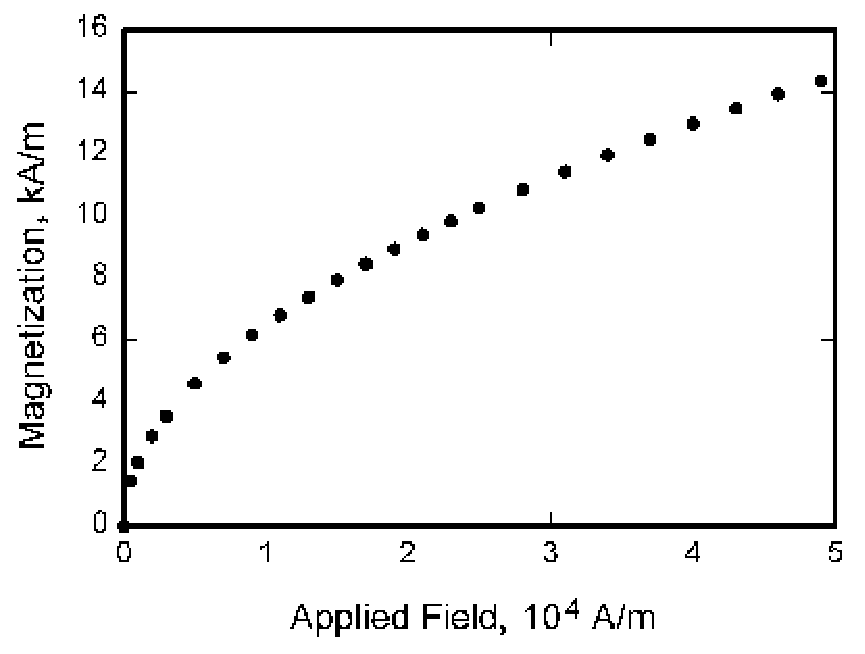
\includegraphics{figure_magnet}
 \caption{Magnetization as a function of applied field, which has
   borders so thick that they overwhelm the data and for some reason the
   ordinate label is rotated 90 degrees to make it difficult to
   read. This figure also demonstrates the dangers of using a bitmap
   as opposed to a vector image.}
 \label{f:magnetic_field}
\end{figure}
Sometimes writing meaningless text can be quiet easy, but other times
one is hard pressed to keep the words flowing.\footnote{And sometimes
things get carried away in endless detail.}
Meanwhile back in the other world, table~\ref{t:scheme_comparison} shows
a nifty comparison.
\begin{table}% no placement specified: defaults to here, top, bottom, page
 \begin{center}
  \caption{Variable and Fixed Coefficient Runge-Kutta Schemes as a
           Function of Reynolds Number}
  \label{t:scheme_comparison}
  \begin{tabular}{rrr}
       Re & Vary & Fixed \\\hline
        1 &  868 & 4,271 \\
       10 &  422 & 2,736 \\
       25 &  252 & 1,374 \\
       50 &  151 &   736 \\
      100 &  110 &   387 \\
      500 &   85 &   136 \\
    1,000 &   77 &   117 \\
    5,000 &   81 &    98 \\
   10,000 &   82 &    99
  \end{tabular}
 \end{center}
\end{table}

\section{Conclusion}

After much typing, the paper can now conclude.
Four rocks were next to the channel.
This caused a few standing waves during the rip that one could ride on
the way in or jump on the way out.

\section*{Appendix}

An appendix, if needed, should appear before the acknowledgments.
Use the 'starred' version of the \verb|\section| commands to avoid
section numbering.

\section*{Acknowledgments}

A place to recognize others.

\begin{thebibliography}{9}% maximum number of references (for label width)
 \bibitem{rebek:82bk}
 Rebek, A., {\it Fickle Rocks}, Fink Publishing, Chesapeake, 1982.
\end{thebibliography}

\end{document}

% - Release $Name:  $ -
